% http://tex.stackexchange.com/questions/30720/footnote-without-a-marker
\newcommand\blfootnote[1]{%
  \begingroup
  \renewcommand\thefootnote{}\footnote{#1}%
  \addtocounter{footnote}{-1}%
  \endgroup
}

\part{Graphics and simulation hardware}
\frame{\partpage}

\begin{frame}{CPUs vs GPUs}
	\begin{itemize}
		\pause \item (CPU = central processing unit; GPU = graphics processing unit)
		\pause \item GPUs are \textbf{highly parallelised}
			\begin{itemize}
				\pause \item Intel i7 6900K: \textbf{8} cores
				\pause \item Nvidia GTX 1080: \textbf{2560} shader processors
			\end{itemize}
		\pause \item GPUs are \textbf{highly specialised}
			\begin{itemize}
				\pause \item Optimised for floating-point calculations rather than logic
				\pause \item Optimised for performing the same calculation on several thousand vertices or pixels at once
			\end{itemize}
	\end{itemize}
\end{frame}

\begin{frame}{Physics processing unit}
	\begin{columns}
		\begin{column}{0.35\textwidth}
			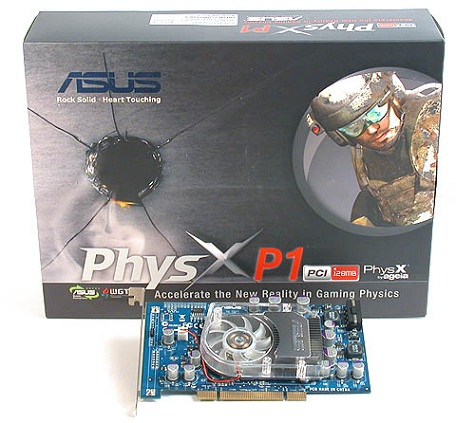
\includegraphics[width=\textwidth]{physx_ppu}
		\end{column}
		\begin{column}{0.63\textwidth}
			\begin{itemize}
				\pause \item Ageia PhysX PPU briefly appeared on the market in 2006-2008
				\pause \item Similar architecture to GPU (many cores, optimised for floating point calculations)
				\pause \item Ageia acquired in 2008 by Nvidia...
				\pause \item Now PhysX is Nvidia's middleware for performing physics simulation on the GPU
			\end{itemize}
		\end{column}
	\end{columns}
\end{frame}

\begin{frame}{General purpose GPU (GPGPU)}
	\begin{itemize}
		\pause \item Early GPUs used a \textbf{fixed pipeline} -- could only be used for rendering 3D graphics
		\pause \item Modern GPUs use a \textbf{programmable pipeline} -- can be programmed for other tasks
		\pause \item Physics simulation (e.g.\ PhysX)
		\pause \item Scientific computing (e.g.\ CUDA)
		\pause \item Deep learning
	\end{itemize}
\end{frame}

\begin{frame}{Graphics APIs}
	\begin{itemize}
		\pause\item Graphics APIs \textbf{abstract} away the differences between different manufacturers' GPUs
		\pause\item There are several APIs in use today:
		\begin{itemize}
			\pause\item \textbf{OpenGL}: Open standard, very mature, very widely supported
			\pause\item \textbf{Vulkan}: Open standard, very new, support still growing
			\pause\item \textbf{Direct3D}: Microsoft only
			\pause\item \textbf{Metal}: Apple only
			\pause\item Sony and Nintendo consoles have their own APIs; Microsoft consoles use Direct3D
		\end{itemize}
		\pause\item Most general-purpose game engines (e.g.\ Unity, Unreal) support several graphics APIs
		\pause\item On this module we will use \textbf{OpenGL} (but the principles are transferable)
	\end{itemize}
\end{frame}
